\documentclass[handout]{beamer}  

%Smaller gap at between top and bottom of block when there are displayed equations
\addtobeamertemplate{block begin}{\setlength\abovedisplayskip{0pt}}
{\setlength{\belowdisplayskip}{0pt}}


\usepackage{setspace}
\linespread{1.3}
\usepackage{amssymb, amsmath, amsthm} 
\usepackage{rotating}
\usepackage{multirow}
\usepackage{graphicx}
\usepackage{synttree}
\usepackage{verbatim}
\usepackage{fancybox}
\usepackage{color}
\usepackage{tikz}
\usetikzlibrary{shapes,backgrounds}
\usepackage{hyperref}
\usetikzlibrary{trees}
\newcommand{\p}{\mathbb{P}}
\newcommand{\expect}{\mathbb{E}}
\newcommand{\var}{\mathbb{V}}



%\setbeamertemplate{blocks}[rounded][shadow=true] 
%gets rid of bottom navigation bars
\setbeamertemplate{footline}{
   \begin{beamercolorbox}[ht=4ex,leftskip=0.3cm,rightskip=0.3cm]{author in head/foot}
%    \usebeamercolor{UniBlue}
    \vspace{0.1cm}
    %\insertshorttitle \ - \insertdate 
    \hfill \insertframenumber / \inserttotalframenumber
   \end{beamercolorbox}
   \vspace*{0.1cm}
} 

%gets rid of navigation symbols
\setbeamertemplate{navigation symbols}{}


%Include or exclude the notes?
%\setbeameroption{show notes}
\setbeameroption{hide notes}


\title[Econ 103]{Economics 103 -- Statistics for Economists} 
\author[F. DiTraglia]{Francis J.\ DiTraglia}
\institute{University of Pennsylvania}
\date{Lecture 14}


\begin{document} 
%%%%%%%%%%%%%%%%%%%%%%%%%%%%%%%%%%%%%%%%

\begin{frame}[plain]
	\titlepage 
	

\end{frame} 

%%%%%%%%%%%%%%%%%%%%%%%%%%%%%%%%%%%%%%%%



\begin{frame}
\begin{center}
\Huge Sampling Distributions and Estimation -- Part I
\end{center}
\end{frame}

%%%%%%%%%%%%%%%%%%%%%%%%%%%%%%%%%%%%%%%%

\begin{frame}
\frametitle{Weighing a Random Sample}
\begin{block}{Bag Contains 100 Candies}
Estimate total weight of candies by weighing a random sample of size 5 and multiplying the result by 20.
\end{block}
\begin{block}{Your Chance to Win}
The bag of candies and a digital scale will make their way around the room \alert{during the lecture}. Each student gets a chance to draw 5 candies and weigh them.
\end{block}
\begin{alertblock}{Student with closest estimate wins the bag of candy!}
\end{alertblock}

\end{frame}
%%%%%%%%%%%%%%%%%%%%%%%%%%%%%%%%%%%%%%%%
\begin{frame}
\frametitle{Weighing a Random Sample}
\begin{block}{Procedure}
When the bag and scale reach your team, do the following:
\end{block}
\begin{enumerate}
\item Fold the top of the bag over and shake to randomize.
\item Randomly draw 5 candies \alert{without replacement}.
\item Weigh your sample and record the result \alert{in grams}.
\item Calculate your \alert{estimate: 20 times the weight of your sample.}
\item Replace your sample and shake again to re-randomize.
\item Pass bag and scale to next student.
\end{enumerate}
\end{frame}


%%%%%%%%%%%%%%%%%%%%%%%%%%%%%%%%%%%%%%%%
\begin{frame}
\frametitle{What is this all about?}

\begin{block}{(Sample) Statistic}
Any function of the data \emph{alone}, e.g.\ sample mean $\bar{x} = \frac{1}{n}\sum_{i=1}^n x_i$
\end{block}

\begin{block}{Statistics}
	\begin{enumerate}
\item Estimation --  Use data to construct educated guess (Estimate) about true value of population parameter. 
\item Inference --  Quantify uncertainty about estimate using:
	\begin{itemize}
	
\item Confidence Intervals
\item Hypothesis Testing 
\end{itemize}

\end{enumerate}
\end{block}

\end{frame}

%%%%%%%%%%%%%%%%%%%%%%%%%%%%%%%%%%%%%%%%
\begin{frame}
\begin{center}
	\Huge How does Probability connect to Statistics?
\end{center}
\end{frame}

%%%%%%%%%%%%%%%%%%%%%%%%%%%%%%%%%%%%%%%%


\begin{frame}
\begin{center}
	\Huge Random Sampling!
\end{center}
\end{frame}

%%%%%%%%%%%%%%%%%%%%%%%%%%%%%%%%%%%%%%%%

\begin{frame}
\frametitle{Random Sampling}

\begin{block}{(Simple) Random Sample}
Select a sample of $n$ objects from a population in such a way that:
	\begin{enumerate}
\item Each member of the population has the same probability of being selected 
\item The fact that one individual is selected does not affect the chance that any other individual is selected
\item Each sample of size $n$ is equally likely to be selected

\end{enumerate}
\end{block}

\end{frame}

%%%%%%%%%%%%%%%%%%%%%%%%%%%%%%%%%%%%%%%%
\begin{frame}
\frametitle{Random Sampling}
In other words:
	$$X_1, X_2, \hdots, X_n \sim \mbox{iid } f(x)$$
is a \alert{Random Sample}

	\vspace{1em}
\begin{block}{Statistics}
Sample is drawn randomly, so sample statistics are \emph{also random}. Use what we know about probability theory to analyze the \emph{distribution} of a statistic under random sampling.
\end{block}
\end{frame}

%%%%%%%%%%%%%%%%%%%%%%%%%%%%%%%%%%%%%%%%
\begin{frame}
\frametitle{Sample with or Without Replacement?}
\pause
Strictly speaking, random samples should be drawn \emph{with replacement}, otherwise there is \emph{dependence}. In practice, this doesn't matter much so long as the population is large relative to the sample. 

\vspace{1em}

\alert{Candy Example In Progress: 100 is large relative to 5.}
\end{frame}
%%%%%%%%%%%%%%%%%%%%%%%%%%%%%%%%%%%%%%%%


\begin{frame}
\frametitle{Estimator versus Estimate}

\begin{block}{Estimator}
An estimator is a function $T(X_1, \hdots, X_n)$ of the random variables we use to represent the random sampling procedure. Hence, it is a random variable itself.
\end{block}
\pause
\begin{block}{Sampling Distribution}
The probability distribution of an Estimator is called a \emph{sampling distribution}.
\end{block}
\pause
\begin{block}{Estimate}
An estimate is a function $T(x_1, \hdots, x_n)$ of the \emph{observed data}, i.e.\ the \emph{realizations} of the random variables we use to represent random sampling. An estimate is a \emph{constant} since the observed data are \emph{constants}
\end{block}

\end{frame}

%%%%%%%%%%%%%%%%%%%%%%%%%%%%%%%%%%%%%%%%


\begin{frame}

\begin{center}
\setlength{\unitlength}{1cm}
\begin{picture}(5,7)
\put(1,6){\framebox(3,1){Population: $f(x)$}}
\pause
\put(4.5,6.5){\makebox{\small \alert{\emph{Probability Distribution}}}}
\pause
\put(2.5,6){\vector(0,-1){1}}
\put(0,3){\framebox(5,1){$X_1, X_2, \hdots, X_n \sim \mbox{iid } f(x)$}}
\put(0.5,4.5){\makebox{\small Random Sample of Size $n$}}
\pause
\put(-3,3.4){\makebox{\small \alert{\emph{Random Variables}}}}
\pause

\put(0.5,3){\vector(-1,-1){1.5}}
\put(-2.3,0.7){\framebox(2.5,0.65){$x_1^{(1)}, \hdots, x_n^{(1)}$}}
\pause

\put(2,3){\vector(0,-1){1.5}}
\put(0.7,0.7){\framebox(2.5,0.65){$x_1^{(2)}, \hdots, x_n^{(2)}$}}

\pause

\put(3.5,2){\makebox{...}}

\pause

\put(4.5,3){\vector(1,-1){1.5}}
\put(4.8,0.7){\framebox(2.5,0.65){$x_1^{(M)}, \hdots, x_n^{(M)}$}}

\put(-1,-0.2){\makebox{\small $M$ Replications, each containing $n$ Observations}}

\pause
\put(5.6,2.6){\makebox{\small \alert{\emph{Realizations}}}}
\put(5.6,2.2){\makebox{\small \alert{\emph{(Constants)}}}}

\end{picture}
\end{center}


\end{frame}
%%%%%%%%%%%%%%%%%%%%%%%%%%%%%%%%%%%%%%%%

\begin{frame}

\begin{center}
\setlength{\unitlength}{1cm}
\begin{picture}(5,7)
\put(-1,5){\framebox(4.5,0.6){$X_1, X_2, \hdots, X_n \sim \mbox{iid } f(x)$}}
\put(-0.7,6){\makebox{\small Random Sample of Size $n$}}

\pause

\put(3.8,5.3){\vector(1,0){1}}
\put(5.5,6){\makebox{\small Estimator}}
\put(5,5){\framebox(2.5,0.6){$T(X_1,\hdots, X_n)$}}

\pause

\put(5,4){\makebox{\small \alert{$\displaystyle\bar{X}_n= \frac{1}{n} \sum_{i=1}^n X_i$}}}

\pause
\put(-2.7,5.6){\makebox{\small \alert{\emph{Random}}}}
\put(-2.7,5.2){\makebox{\small \alert{\emph{Variables}}}}


\pause

\put(1.2,4.7){\vector(0,-1){2.3}}
\put(-0.2,1.7){\makebox{\small Observations (Data)}}
\put(0,0.7){\framebox(2.5,0.6){$x_1, \hdots, x_n$}}

\pause

\put(4.5,1.7){\makebox{\small Estimate}}
\put(4,0.7){\framebox(2.5,0.6){$T(x_1, \hdots, x_n)$}}
\put(2.8,1){\vector(1,0){1}}


\pause

\put(4,-0.2){\makebox{\small \alert{$\displaystyle\bar{x}= \frac{1}{n} \sum_{i=1}^n x_i$}}}

\pause

\put(-2.7,0.9){\makebox{\small \alert{\emph{Constants}}}}
\end{picture}
\end{center}


\end{frame}
%%%%%%%%%%%%%%%%%%%%%%%%%%%%%%%%%%%%%%%%



\begin{frame}
\frametitle{Population: All Students in the Class}
\begin{center}
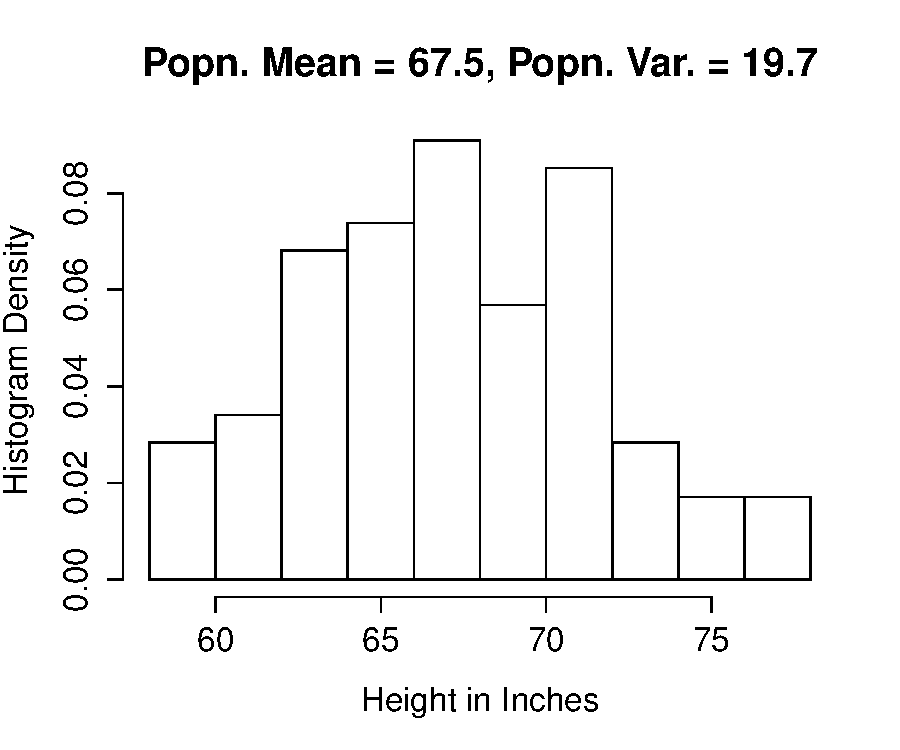
\includegraphics[scale = 0.54]{./images/height_hist}
\end{center}
\end{frame}
%%%%%%%%%%%%%%%%%%%%%%%%%%%%%%%%%%%%%%%%


\begin{frame}

\begin{center}
\setlength{\unitlength}{1cm}
\begin{picture}(5,7)
\put(0,5){\framebox(5,1){$X_1, X_2, \hdots, X_n \sim \mbox{iid } f(x)$}}
\put(0.5,6.5){\makebox{\small Random Sample of Size $n$}}

\pause

\put(0.5,5){\vector(-1,-1){1.5}}
\put(-2.3,2.7){\framebox(2.5,0.65){$x_1^{(1)}, \hdots, x_n^{(1)}$}}

\pause

\put(-1,2.5){\vector(0,-1){1}}
\put(-1.1,0.9){\makebox{\small $\bar{x}_1$}}

\pause

\put(2,5){\vector(0,-1){1.5}}
\put(0.7,2.7){\framebox(2.5,0.65){$x_1^{(2)}, \hdots, x_n^{(2)}$}}

\pause

\put(2,2.5){\vector(0,-1){1}}
\put(1.9,0.9){\makebox{\small $\bar{x}_2$}}

\pause

\put(3.8,3){\makebox{...}}
\put(3.8,1){\makebox{...}}

\pause

\put(4.5,5){\vector(1,-1){1.5}}
\put(4.8,2.7){\framebox(2.5,0.65){$x_1^{(M)}, \hdots, x_n^{(M)}$}}

\pause

\put(6,2.5){\vector(0,-1){1}}
\put(5.9,0.9){\makebox{\small $\bar{x}_M$}}

\pause

\put(-0.5,0){\makebox{\small $M$ Replications yield $M$ \emph{different estimates}}}

\pause

\put(-0.5,-0.6){\makebox{\small \alert{Sampling Distribution: Infinite Replications}}}

\end{picture}
\end{center}


\end{frame}
%%%%%%%%%%%%%%%%%%%%%%%%%%%%%%%%%%%%%%%%

\begin{frame}
\frametitle{Histograms of sampling distribution of sample mean $\bar{X}_n$}
\alert{Random Sampling With Replacement, 10000 Reps. Each}
\begin{center}
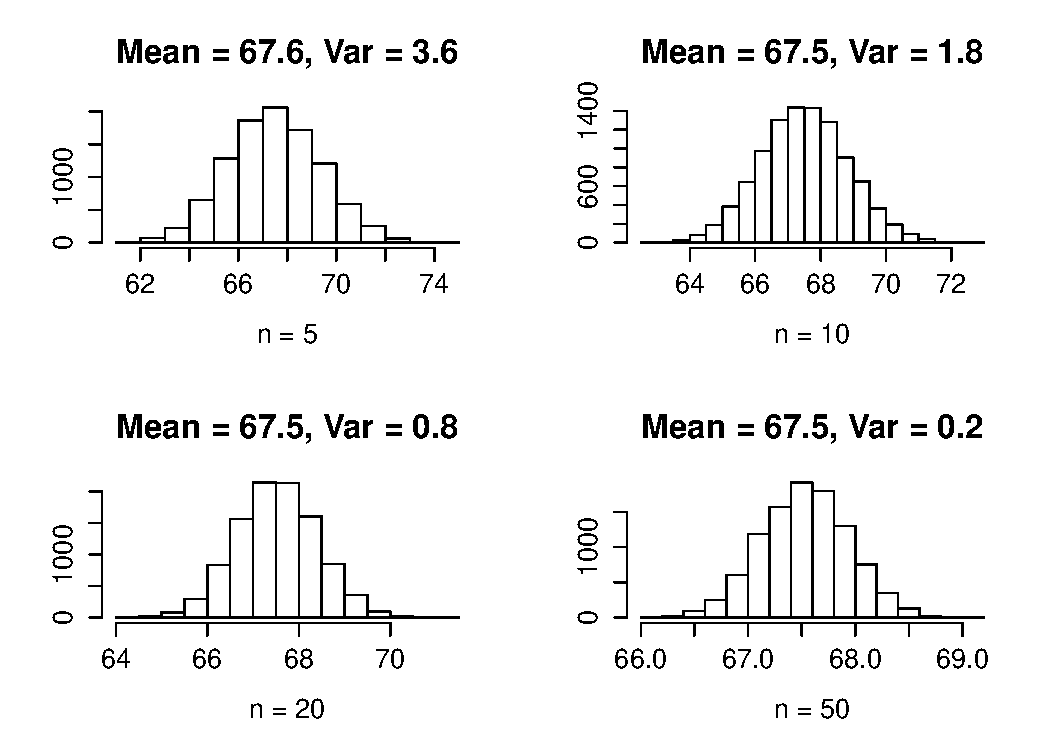
\includegraphics[scale = 0.55]{./images/height_samples}
\end{center}
\end{frame}
%%%%%%%%%%%%%%%%%%%%%%%%%%%%%%%%%%%%%%%%
\begin{frame}
\frametitle{Population Distribution vs.\ Sampling Distribution of $\bar{X}_n$}

\begin{columns} 
\begin{column}[c]{6cm} 

 %FIRST COLUMN HERE 
\begin{figure}
\centering
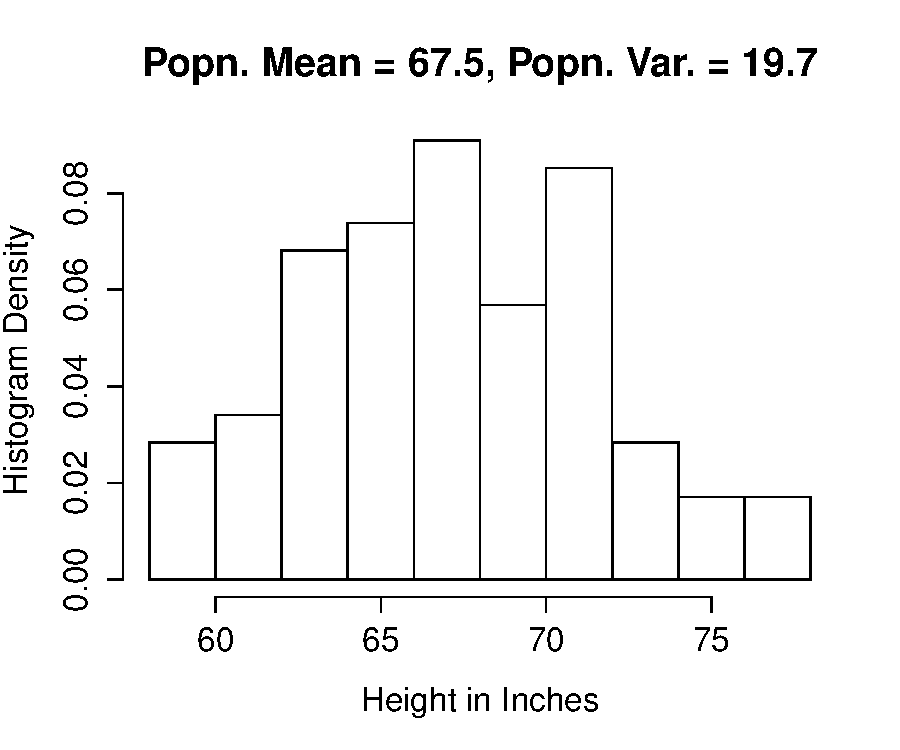
\includegraphics[scale = 0.35]{./images/height_hist}
\end{figure}
\end{column} 
\begin{column}[c]{6cm} 

 %SECOND COLUMN HERE 
 \small
\begin{table}
\begin{tabular}{|rrr|}
\hline
&\multicolumn{2}{c|}{Sampling Dist.\ of $\bar{X}_n$}\\
$n$&Mean&Variance\\
\hline
5&67.6&3.6\\
10&67.5&1.8\\
20&67.5&0.8\\
50&67.5&0.2\\
\hline
\end{tabular}
\end{table}

\end{column} 
\end{columns} 
\begin{alertblock}{Two Things to Notice:}
\begin{enumerate}
	\item Sampling dist.\ ``correct on average'' 
	\item Sampling variability decreases with $n$
\end{enumerate}
\end{alertblock}
\end{frame}

%%%%%%%%%%%%%%%%%%%%%%%%%%%%%%%%%%%%%%%%
\begin{frame}
\frametitle{$X_1,\hdots, X_{9} \sim \mbox{ iid }$ with $\mu=5$, $\sigma^2 =36$. \hfill
\includegraphics[scale = 0.05]{./images/clicker}}

\large Calculate:
	 $$E(\bar{X}) = E\left[\frac{1}{9}(X_1 + X_2 + \hdots + X_{9})\right]$$
\end{frame}
%%%%%%%%%%%%%%%%%%%%%%%%%%%%%%%%%%%%%%%%
\begin{frame}
\frametitle{Mean of Sampling Distribution of $\bar{X}_n$}
\alert{$X_1, \hdots, X_n \sim \mbox{iid with mean }\mu$}
\begin{eqnarray*}
E[\bar{X_n}] = E\left[ \frac{1}{n}\sum_{i=1}^n X_i \right]\pause = \frac{1}{n} \sum_{i=1}^n E[X_i] = \pause\frac{1}{n} \sum_{i=1}^n \mu = \pause \frac{n\mu}{n} =\pause \mu
\end{eqnarray*}
\pause \alert{Hence, sample mean is ``correct on average.'' The formal term for this is \emph{unbiased}.}
\end{frame}

%%%%%%%%%%%%%%%%%%%%%%%%%%%%%%%%%%%%%%%%
\begin{frame}
\frametitle{$X_1,\hdots, X_{9} \sim \mbox{ iid }$ with $\mu=5$, $\sigma^2 = 36$. \hfill
\includegraphics[scale = 0.05]{./images/clicker}}

\large Calculate:
	 $$Var(\bar{X}) = Var\left[\frac{1}{9}(X_1 + X_2 + \hdots + X_{9})\right]$$
\end{frame}
%%%%%%%%%%%%%%%%%%%%%%%%%%%%%%%%%%%%%%%%

\begin{frame}
\frametitle{Variance of Sampling Distribution of $\bar{X}_n$}
\alert{$X_1, \hdots, X_n \sim \mbox{iid with mean }\mu \mbox{ and variance } \sigma^2$}
\begin{eqnarray*}
Var[\bar{X_n}] &=& Var\left[ \frac{1}{n}\sum_{i=1}^n X_i \right] \pause= \frac{1}{n^2} \sum_{i=1}^n Var(X_i) \\
&=& \pause \frac{1}{n^2} \sum_{i=1}^n \sigma^2 = \pause \frac{n\sigma^2}{n^2} = \pause \frac{\sigma^2}{n}
\end{eqnarray*}
\pause
\alert{Hence the variance of the sample mean \emph{decreases linearly with sample size}.}
\end{frame}
%%%%%%%%%%%%%%%%%%%%%%%%%%%%%%%%%%%%%%%%
\begin{frame}
\frametitle{$X_1,\hdots, X_{9} \sim \mbox{ iid }$ with $\mu=5$, $\sigma^2 = 36$. \hfill
\includegraphics[scale = 0.05]{./images/clicker}}

\large Calculate:
	 $$SD(\bar{X}) = SD\left[\frac{1}{9}(X_1 + X_2 + \hdots + X_{9})\right]$$
\end{frame}
%%%%%%%%%%%%%%%%%%%%%%%%%%%%%%%%%%%%%%%%
\begin{frame}
\frametitle{Standard Error}
Std. Dev.\ of estimator's sampling dist.\ is called \alert{standard error}.
\begin{block}{Standard Error of the Sample Mean}
$SE(\bar{X}_n)= \sqrt{Var\left(\bar{X}_n\right)}= \sqrt{\sigma^2/n}=\sigma/\sqrt{n}$
\end{block}
\end{frame}
%%%%%%%%%%%%%%%%%%%%%%%%%%%%%%%%%%%%%%%%

\begin{frame}

\begin{center}
\huge Why $(n-1)$ for sample variance?
\end{center}

\end{frame}
%%%%%%%%%%%%%%%%%%%%%%%%%%%%%%%%%%%%%%%%

\begin{frame}
\frametitle{Why $(n-1)$ for sample variance?}
\alert{We will show that having $n-1$ in the denominator ensures:}
$$E[S^2] =E\left[ \frac{1}{n-1} \sum_{i=1}^n \left(X_i - \bar{X}\right)^2\right] = \sigma^2$$
\alert{under random sampling.}
\end{frame}


%%%%%%%%%%%%%%%%%%%%%%%%%%%%%%%%%%%%%%%%

\begin{frame}
\frametitle{Why $(n-1)$ for sample variance?}
\begin{block}{Step \# 1 -- Tedious but straightforward algebra gives:}
	$$\sum_{i=1}^n \left(X_i - \bar{X}\right)^2 = \left[  \sum_{i=1}^n \left(X_i - \mu\right)^2\right] - n(\bar{X}-\mu)^2$$
\end{block}
\alert{You are not responsible for proving Step \#1 on an exam.}

\end{frame}
%%%%%%%%%%%%%%%%%%%%%%%%%%%%%%%%%%%%%%%%
\begin{frame}
\scriptsize
\begin{eqnarray*}
	\sum_{i=1}^n \left(X_i - \bar{X}\right)^2 &=& \sum_{i=1}^n \left(X_i - \mu + \mu - \bar{X}\right)^2 = \sum_{i=1}^n \left[(X_i -\mu) - (\bar{X} - \mu)\right]^2\\
		&=&\sum_{i=1}^n \left[(X_i -\mu)^2 - 2(X_i -\mu)(\bar{X} - \mu) + (\bar{X} - \mu)^2\right]\\
		&=&\sum_{i=1}^n (X_i -\mu)^2 - \sum_{i=1}^n 2(X_i -\mu)(\bar{X} - \mu) + \sum_{i=1}^n (\bar{X} - \mu)^2\\
		&=& \left[  \sum_{i=1}^n \left(X_i - \mu\right)^2\right]   - 2(\bar{X} - \mu) \sum_{i=1}^n (X_i -\mu)+n(\bar{X} - \mu)^2\\
				&=& \left[  \sum_{i=1}^n \left(X_i - \mu\right)^2\right]   - 2(\bar{X} - \mu) \left( \sum_{i=1}^n X_i- \sum_{i=1}^n \mu \right)+n(\bar{X} - \mu)^2\\
				&=& \left[  \sum_{i=1}^n \left(X_i - \mu\right)^2\right]   - 2(\bar{X} - \mu)(n\bar{X}-n\mu)+n(\bar{X} - \mu)^2\\
				&=&\left[  \sum_{i=1}^n \left(X_i - \mu\right)^2\right]   - 2n(\bar{X} - \mu)^2+n(\bar{X} - \mu)^2\\
				&=&\left[  \sum_{i=1}^n \left(X_i - \mu\right)^2\right]   - n(\bar{X} - \mu)^2
\end{eqnarray*}
\end{frame}

%%%%%%%%%%%%%%%%%%%%%%%%%%%%%%%%%%%%%%%%

\begin{frame}
\frametitle{Why $(n-1)$ for sample variance?}
\begin{block}{Step \# 2 -- Take Expectations of Step \# 1:}
	\begin{eqnarray*}
		E\left[\sum_{i=1}^n \left(X_i - \bar{X}\right)^2\right] &=& E\left[\left\{  \sum_{i=1}^n \left(X_i - \mu\right)^2\right\} - n(\bar{X}-\mu)^2\right]\\
			&=&\pause E\left[ \sum_{i=1}^n \left(X_i - \mu\right)^2\right] -E\left[ n(\bar{X}-\mu)^2\right]\\
			&=&\pause  \sum_{i=1}^n E\left[\left(X_i - \mu\right)^2\right] -n\;E\left[ (\bar{X}-\mu)^2\right]\\
	\end{eqnarray*}
\end{block}
\alert{Where we have used the linearity of expectation.}
\end{frame}
%%%%%%%%%%%%%%%%%%%%%%%%%%%%%%%%%%%%%%%%


\begin{frame}
\frametitle{Why $(n-1)$ for sample variance?}
\begin{block}{Step \# 3 -- Use assumption of random sampling:}
\alert{$X_1, \hdots, X_n \sim \mbox{ iid}$ with mean $\mu$ and variance $\sigma^2$}
	\begin{eqnarray*}
		E\left[\sum_{i=1}^n \left(X_i - \bar{X}\right)^2\right] &=&  \sum_{i=1}^n E\left[\left(X_i - \mu\right)^2\right] -n\;E\left[ (\bar{X}-\mu)^2\right]\\
		&=&  \pause \sum_{i=1}^n Var(X_i) -n\;E\left[ (\bar{X}-E[\bar{X}])^2\right]\\
		&=& \pause   \sum_{i=1}^n Var(X_i) -n\;Var(\bar{X})= n\sigma^2 - \sigma^2\\
		&=& \pause (n-1)\sigma^2
	\end{eqnarray*}
\end{block}
\alert{Since we showed earlier today that  $E[\bar{X}]=\mu$ and $Var(\bar{X})=\sigma^2/n$ under this random sampling assumption.}
\end{frame}
%%%%%%%%%%%%%%%%%%%%%%%%%%%%%%%%%%%%%%%%

\begin{frame}
\frametitle{Why $(n-1)$ for sample variance?}
\begin{block}{Finally -- Divide Step \# 3 by $(n-1)$:}
	\begin{eqnarray*}
		E[S^2] &=& E\left[\frac{1}{n-1}\sum_{i=1}^n \left(X_i - \bar{X}\right)^2\right]= \frac{(n-1)\sigma^2}{n-1} = \sigma^2
	\end{eqnarray*}
\end{block}
\alert{Hence, having $(n-1)$ in the denominator ensures that the sample variance is ``correct on average,'' that is \emph{unbiased}.}
\end{frame}
%%%%%%%%%%%%%%%%%%%%%%%%%%%%%%%%%%%%%%%%

% \begin{frame}
% \frametitle{Unbiased means ``Right on Average''}

% \begin{block}{Bias of an Estimator}
% Let $\widehat{\theta}_n$ be a sample estimator of a population parameter $\theta_0$. The \emph{bias} of $\widehat{\theta}_n$ is $E[\widehat{\theta}_n] - \theta_0$.
% \end{block}

% \begin{block}{Unbiased Estimator}
% A sample estimator $\widehat{\theta}_n$ of a population parameter $\theta_0$ is called \emph{unbiased} if $E[\widehat{\theta}_n]= \theta_0$
% \end{block}

% \end{frame}


%%%%%%%%%%%%%%%%%%%%%%%%%%%%%%%%%%%%%%%%


\end{document}